\documentclass[]{jsarticle}
\usepackage[dvipdfmx]{graphicx}
\usepackage{comment}
\usepackage{listings,jvlisting}
\usepackage{verbatim}
\usepackage{url}
\usepackage[utf8]{inputenc}
\usepackage{float}

\lstset{
  basicstyle={\ttfamily},
  identifierstyle={\small},
  commentstyle={\smallitshape},
  keywordstyle={\small\bfseries},
  ndkeywordstyle={\small},
  stringstyle={\small\ttfamily},
  frame={tb},
  breaklines=true,
  columns=[l]{fullflexible},
  numbers=left,
  xrightmargin=0zw,
  xleftmargin=2zw,
  numberstyle={\scriptsize},
  stepnumber=1,
  numbersep=1zw,
  lineskip=-0.5ex,
}
\renewcommand{\lstlistingname}{ソースコード}
\title{\vspace{-3cm} \textbf{プログラミング言語実験・C言語 第4回課題レポート}}
\author{\textbf{I類 メディア情報学} \\\textbf{氏名:}LEORA DAVID\\\textbf{学籍番号:}2210745}
\date{\textbf{2024年05月10日}}

\begin{document}
\maketitle

\section{課題7(階段出し機能の実装)}
コンピュータ大貧民教育用クライアント(tndhmc-0.03.tar.gz)のディレクトリ src にある、 select\_cards.c などを改変し、
階段出し機能を実現した。
この課題では、場にカードがない状況で、 かつ提出するカードにジョーカーを含まない場合について実装した。\\

実装が完了したら、大貧民サーバを立ち上げゲームを実行し、 階段出しが行われている様子がわかるスクリーンショットを取得して、図1に示した。具体的には、コードの一部を変更して、ソースコード1とソースコード2に示す。
また、実現した階段出し機能について、考察を行った。

\begin{lstlisting}[caption={daihinmin.c}]
  void make_info_table(int info_table[8][15], int my_cards[8][15])
  {
    int i, j;

    clear_table(info_table);
    for (i = 0; i < 4; i++)
    {
      for (j = 13; j > 0; j--)
      {
        if (my_cards[i][j] == 1)
          info_table[i][j] = info_table[i][j + 1] + 1;
        else if (my_cards[i][j] == 0)
          info_table[i][j] = 0;
      }
    }

    for (i = 0; i < 4; i++)
    {
      for (j = 1; j < 14; j++)
      {
        if (info_table[i][j] == 2)
          info_table[i][j] = 1;
      }
    }

    for (i = 1; i <= 13; i++)
    {
      info_table[4][i] = my_cards[0][i] + my_cards[1][i] + my_cards[2][i] + my_cards[3][i];
    }
  }

  int search_low_sequence(int dst_cards[8][15], int info_table[8][15])
  {
    int i, j, k;
    int search_flag = 0;
    clear_table(dst_cards);
    for (i = 1; i <= 13; i++)
    {
      for (j = 0; j < 4; j++)
      {
        if (info_table[j][i] >= 3)
        {
          search_flag = 1;
          break;
        }
      }
      if (search_flag == 1)
        break;
    }
    if (i <= 13)
    {
      for (k = 0; k < info_table[j][i]; k++)
      {
        dst_cards[j][i + k] = 1;
      }
    }
    return 0;
  }
\end{lstlisting}



\begin{lstlisting}[caption={select\_cards.c}]
  void select_cards_free(int select_cards[8][15], int my_cards[8][15], state *field_status)
  {
    int info_table[8][15];
  
    make_info_table(info_table, my_cards);
    if (count_cards(select_cards) == 0)
      search_low_sequence(select_cards, info_table); // 手持ちの一番弱い階段を提出する
    if (count_cards(select_cards) == 0)
      search_low_pair(select_cards, info_table, my_cards); // 手持ちの一番弱いペアを提出する
    if (count_cards(select_cards) == 0)
      search_low_card(select_cards, my_cards, 0); // 手持ちの一番弱いカードを単騎で提出する
  }
\end{lstlisting}

\section*{課題7の考察}
ソースコード1によると、まず、make\_info\_table関数は、手札の情報を元に、階段やペアの情報を格納した配列を作成する。
やり方としては、make\_info\_table 関数では手札の情報を一番右から左に、各スートごとのカードの連続した枚数を数え、それを配列に格納する。
カードを持っていない場合は、0を格納する。また、配列の中に2が格納されているマスがある場合、それを1として格納する。これは、この後のジョーカーが利用されるかどうかのために設定される。\\

その後、search\_low\_sequence関数は、make\_info\_table関数で作成した配列を元に、階段を探す関数である。
search\_low\_sequence関数では、配列の中に一番左から最初に3以上連続したカードがある場合、それを提出するようにしている。
流れとしては、for ループで配列を探し、見つかった場合はフラグを立て、ループを break する。
その後、見つかった場合は、そのマスから何枚数連続しているカードを右に探し、dst\_cardsに格納してそれを提出するようにしている。\\

また、ソースコード2によると、select\_cards.cのselect\_cards\_free関数では、場にカードがない場合、階段を提出するようにしている。
もし、提出する階段がない場合は、ペアを提出し、それもない場合は、一番弱い単騎のカードを提出するようにしている。

\newpage
\section*{課題7の実行結果}
階段出し機能の実装結果を図1に示す。図1を見ると、場にカードがない状況で、かつ提出するカードにジョーカーを含まない場合に、階段出し機能が実装されていることがわかる。
今回は、クローバーの「3」、「4」、「5」が場が空の状況で階段として提出されることを確認した。\\
\begin{figure}[h]
  \centering
  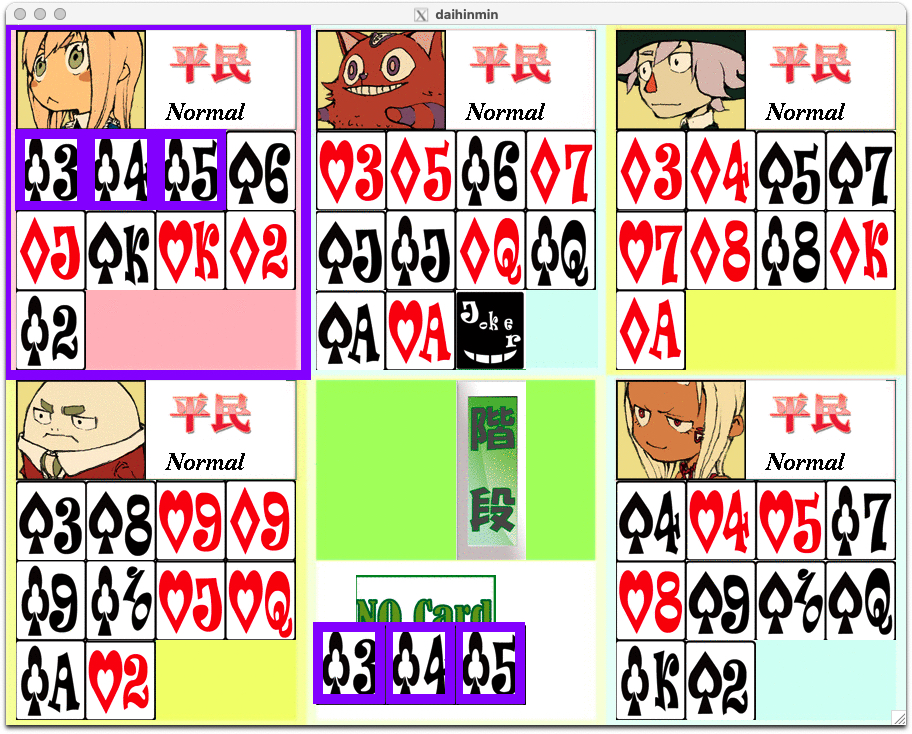
\includegraphics[width=0.8\textwidth]{./kadai7kaidan.jpg}
  \caption{階段出し機能の実装}
\end{figure}

\newpage
\section{課題8(場にカードが出ている場合に対するペア出し機能と階段出し機能の実装)}
課題6および課題7のプログラムを改良し、 「場にカードが出ている場合」に対するペア出し機能と階段出し機能を実現した。
なお、提出するカードにジョーカーを含まない場合について実装した。\\

実装が完了したら、大貧民サーバを立ち上げゲームを実行し、 場にカードが出ている状態からペア出しや階段出しが行われている様子がわかる
スクリーンショットを取得して、図2と図3に示した。
また、実現したペア出し機能や階段出し機能について、考察を行った。\\

\begin{lstlisting}[caption={select\_cards.c}]
  void select_cards_restrict(int select_cards[8][15], int my_cards[8][15], state *field_status)
{
  int tmp_cards[8][15];
  copy_table(tmp_cards, my_cards);

  int info_table[8][15];
  if (field_status->is_sequence == 1)
  { // 場が階段のとき
    if (field_status->is_lock == 1)
    { // 場が縛られている
      remove_suit(tmp_cards, field_status->suit, 1);
      remove_low_card(tmp_cards, field_status->order, 0);
      make_info_table(info_table, my_cards);
      search_low_sequence(select_cards, info_table);
    }
    else
    { // 場が縛られていない
      remove_low_card(tmp_cards, field_status->order, 0);
      make_info_table(info_table, my_cards);
      search_low_sequence(select_cards, info_table);
    }
  }
  else if (field_status->quantity > 1)
  { // 場がペアのとき
    if (field_status->is_lock == 1)
    { // 場が縛られている
      remove_suit(tmp_cards, field_status->suit, 1);
      remove_low_card(tmp_cards, field_status->order, 0);
      make_info_table(info_table, my_cards);
      search_low_pair(select_cards, info_table, tmp_cards);
    }
    else
    { // 場が縛られていない
      remove_low_card(tmp_cards, field_status->order, 0);
      make_info_table(info_table, my_cards);
      search_low_pair(select_cards, info_table, tmp_cards);
    }
  }
  else
  { // 場が単騎のとき
    if (field_status->is_lock == 1)
    { // 場が縛られている
      remove_suit(tmp_cards, field_status->suit, 1);
      remove_low_card(tmp_cards, field_status->order, 0);
      search_low_card(select_cards, tmp_cards, 1);
    }
    else
    { // 場が縛られていない
      remove_low_card(tmp_cards, field_status->order, 0);
      search_low_card(select_cards, tmp_cards, 1);
    }
  }
}
\end{lstlisting}

\section*{課題8の考察}
ソースコード3によると、関数 select\_cards\_restrict は、場にカードが出ている場合に対するペア出し機能と階段出し機能や単騎カードを出す機能を実現している。
また、それぞれの場合によって、場が縛られているかどうかによって、処理を変えている。
まず、階段出し機能の場合については、場が縛られているとき、remove\_suit関数を使って、場のスートと同じスートのカードを取り除き、それ以下のカードを取り除いてから、info\_tableを作成し、search\_low\_sequence関数を呼び出している。
一方、場が縛られていない時は、remove\_suit関数を使わずに、remove\_low\_card関数を使って、場のカードよりも小さいカードを取り除いてから、info\_tableを作成し、search\_low\_sequence関数を呼び出している。
これは、場が縛られている場合は、他のスートのカードを出せないため、場のスートと同じスートのカードだけを取り除いている。\\

\indent また、ペア出し機能の場合についても、同様に場が縛られているかどうかによって処理を変えている。
場が縛られている場合は、remove\_suit関数を使って、場のスートと同じスートのカードを取り除き、それ以下のカードを取り除いてから、info\_tableを作成し、search\_low\_pair関数を呼び出している。
一方、場が縛られていない時は、remove\_low\_card関数を使って、場のカードよりも小さいカードを取り除いてから、info\_tableを作成し、search\_low\_pair関数を呼び出している。
最後に、単騎カードを出す機能の場合についても、同様に場が縛られているかどうかによって処理を変えている。

\newpage
\section*{課題8の実行結果}
場にカードが出ている場合に対する\textbf{ペア出し機能}の実装結果を図2に示す。図2を見ると、場にカードが出ている状況で、かつ提出するカードにジョーカーを含まない場合に、ペア出し機能が実装されていることがわかる。\\
\begin{figure}[h]
  \centering
  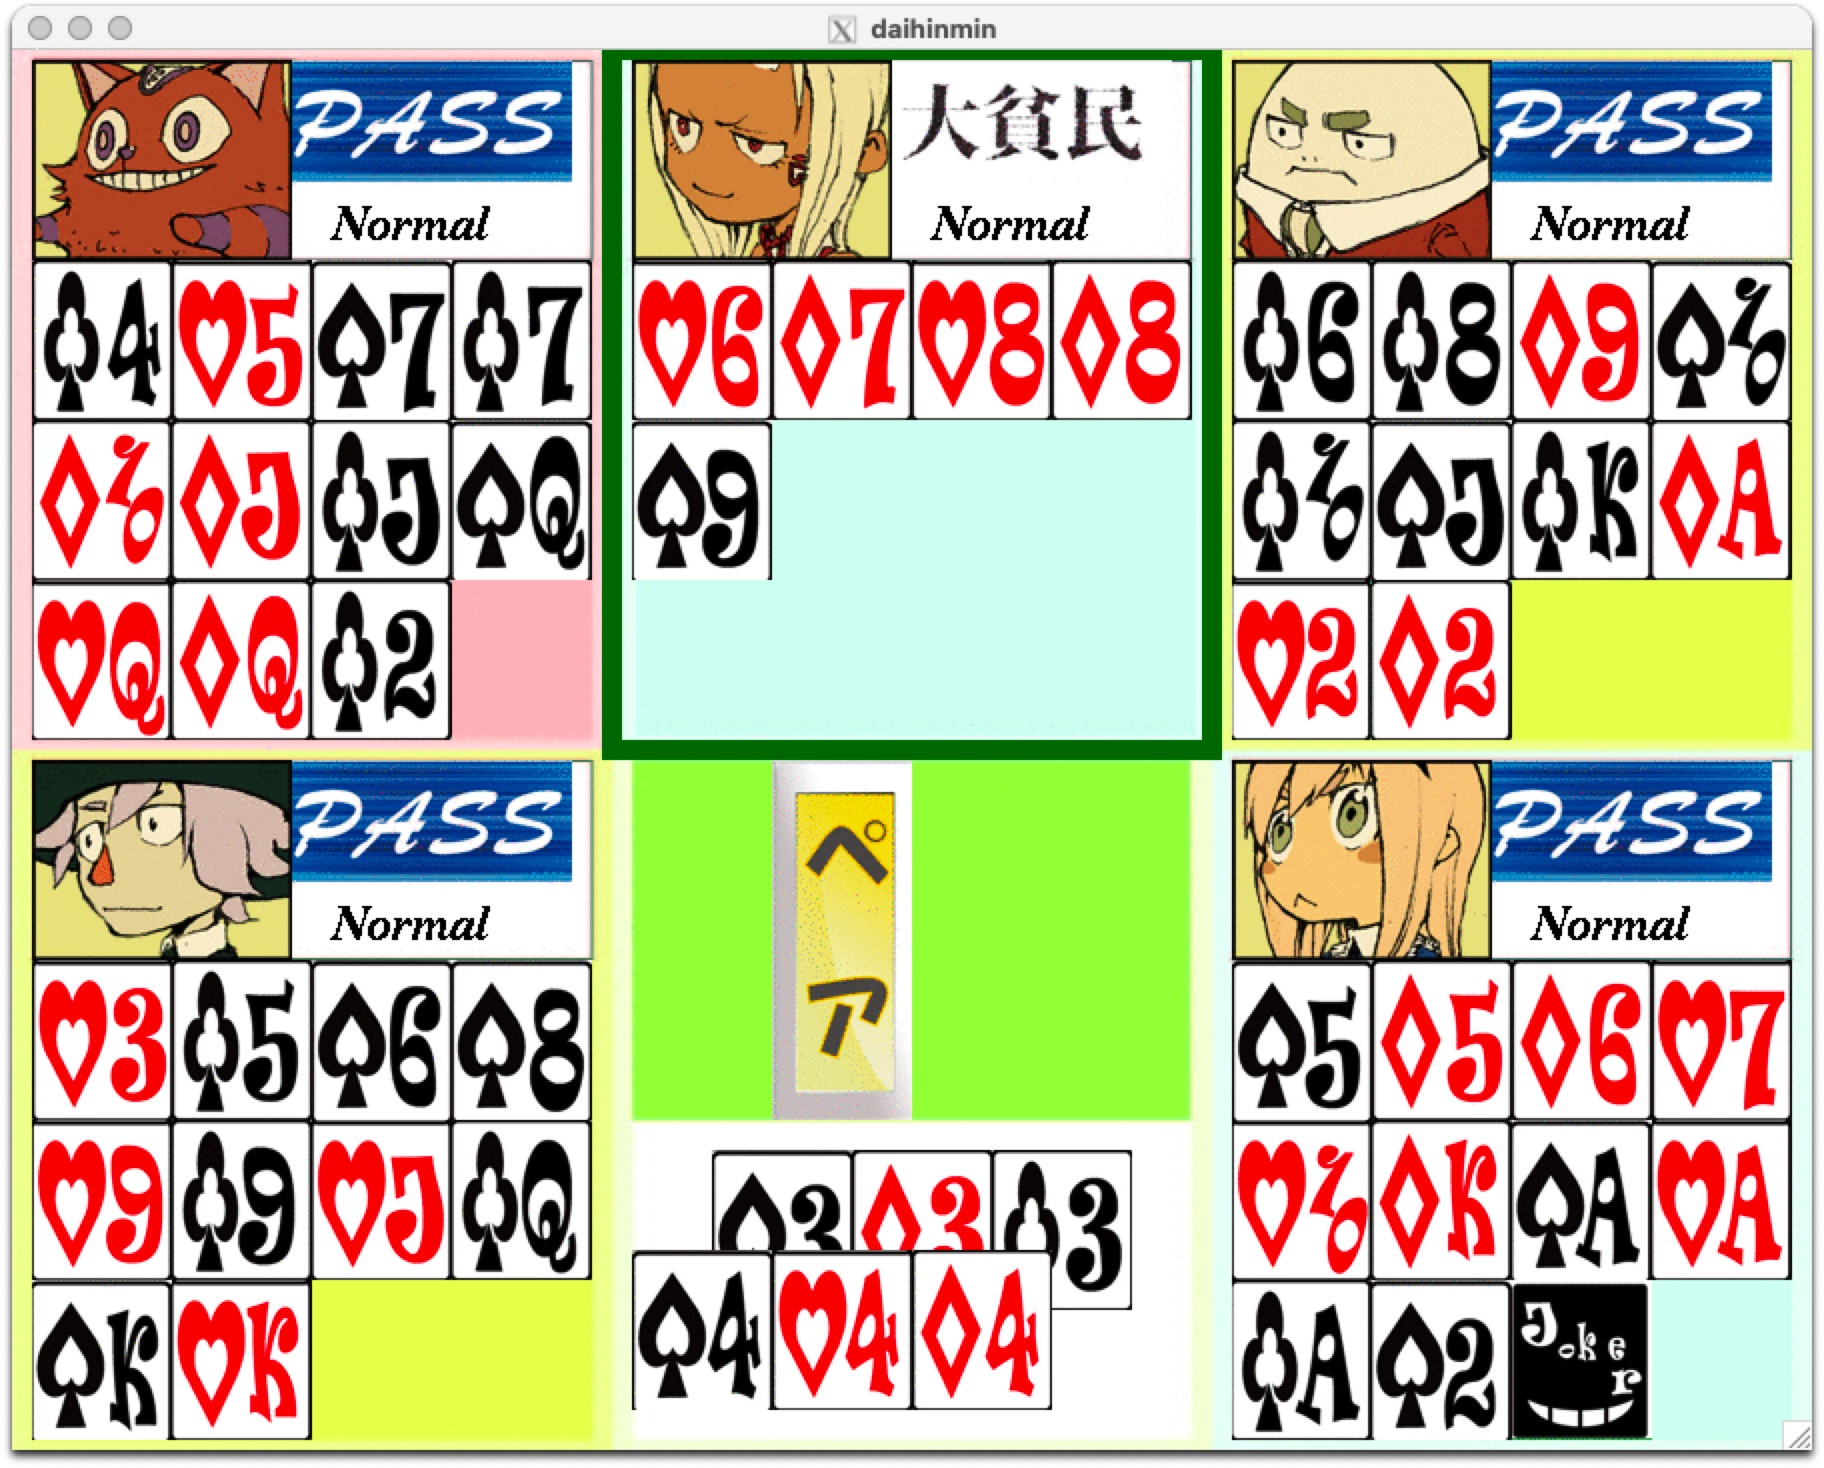
\includegraphics[width=0.8\textwidth]{./kadai8pair.jpg}
  \caption{場にカードが出ている場合に対するペア出し機能の実装結果}
\end{figure}
\newpage
また、場にカードが出ている場合に対する\textbf{階段出し機能}の実装結果を図3に示す。図3を見ると、場にカードが出ている状況で、かつ提出するカードにジョーカーを含まない場合に、階段出し機能が実装されていることがわかる。\\
\begin{figure}[h]
  \centering
  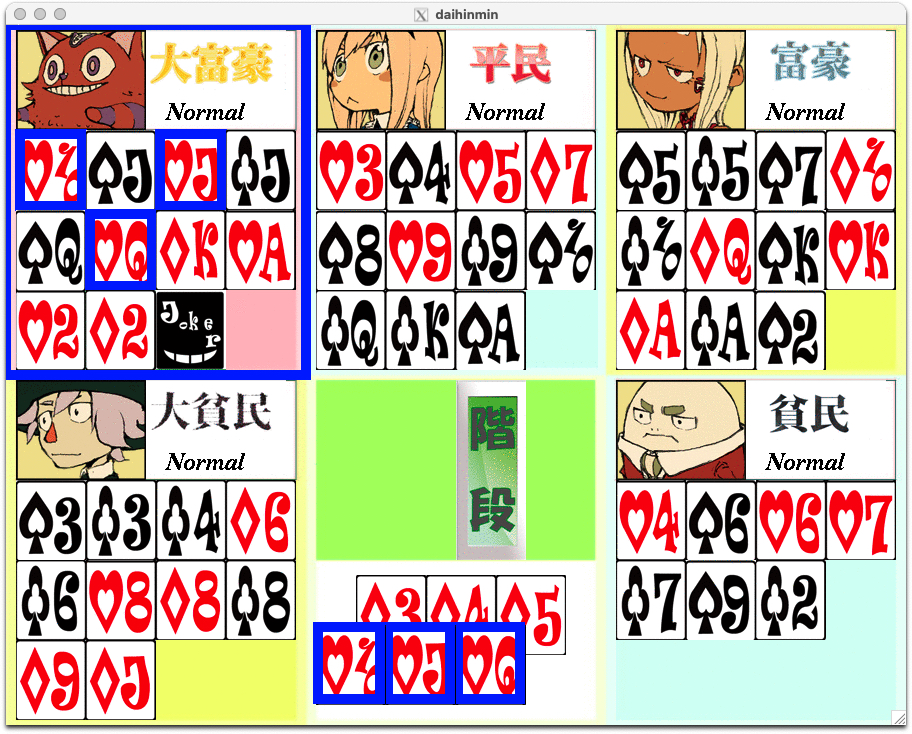
\includegraphics[width=0.8\textwidth]{./kadai8kaidan2.jpg}
  \caption{場にカードが出ている場合に対する階段出し機能の実装結果}
\end{figure}

\newpage
\section{課題9(ペアや階段として出せるカードの温存)}
コンピュータ大貧民教育用クライアント(tndhmc-0.03.tar.gz)のディレクトリ src にある、 daihinmin.c などを改変し、
ペアや階段として出せるカードを温存する機能を実現した。\\

実装が完了したら、大貧民サーバを立ち上げゲームを実行し、 カードを温存している様子がわかるスクリーンショットを取得して、図4と図5に示した。
また、実現したカードの温存機能について、考察を行った。

\begin{lstlisting}[caption={daihinmin.c}]
  void search_low_card_wosp(int out_cards[8][15], int my_cards[8][15], int info_table[8][15], int use_joker_flag){
    int i, j, find_flag = 0;
  
    clear_table(out_cards);
    for (j = 1; j < 14 && find_flag == 0; j++)
    {
      for (i = 0; i < 4 && find_flag == 0; i++)
      {
        if (my_cards[i][j] == 1 && info_table[4][j] == 1)
        {
          find_flag = 1;
          out_cards[i][j] = my_cards[i][j];
        }
      }
    }
    if (find_flag == 0 && use_joker_flag == 1)
    {
      out_cards[0][14] = 2;
    }
  }
\end{lstlisting}

\begin{lstlisting}[caption={select\_cards.c}]
  void select_cards_restrict(int select_cards[8][15], int my_cards[8][15], state *field_status)
  {
    int tmp_cards[8][15];
    copy_table(tmp_cards, my_cards);
    int info_table[8][15];
  
    if (field_status->is_sequence == 1)
    { // 場が階段のとき
      if (field_status->is_lock == 1)
      { // 場が縛られている
        remove_suit(tmp_cards, field_status->suit, 1);
        remove_low_card(tmp_cards, field_status->order, 0);
        make_info_table(info_table, my_cards);
        search_low_sequence(select_cards, info_table);
      }
      else
      { // 場が縛られていない
        remove_low_card(tmp_cards, field_status->order, 0);
        make_info_table(info_table, my_cards);
        search_low_sequence(select_cards, info_table);
      }
    }
    else if (field_status->quantity > 1)
    { // 場がペアのとき
      if (field_status->is_lock == 1)
      { // 場が縛られている
        remove_suit(tmp_cards, field_status->suit, 1);
        remove_low_card(tmp_cards, field_status->order, 0);
        make_info_table(info_table, my_cards);
        search_low_pair(select_cards, info_table, tmp_cards);
      }
      else
      { // 場が縛られていない
        remove_low_card(tmp_cards, field_status->order, 0);
        make_info_table(info_table, my_cards);
        search_low_pair(select_cards, info_table, tmp_cards);
      }
    }
    else
    { // 場が単騎のとき
      if (field_status->is_lock == 1)
      { // 場が縛られている
        remove_suit(tmp_cards, field_status->suit, 1);
        remove_low_card(tmp_cards, field_status->order, 0);
        make_info_table(info_table, my_cards);
        search_low_card_wosp(select_cards, tmp_cards, info_table, 1);
      }
      else
      { // 場が縛られていない
        remove_low_card(tmp_cards, field_status->order, 0);
        make_info_table(info_table, my_cards);
        search_low_card_wosp(select_cards, tmp_cards, info_table, 1);
      }
    }
  }
\end{lstlisting}

\section*{課題9の考察}
ソースコード4によると、search\_low\_card\_wosp関数を新しく作成して、ペアや階段として出せるカードを温存する機能を実現している。
やり方としては、search\_low\_card関数と似ていますが、その中に、my\_cards配列の中のカード枚数が1で、info\_table配列の5行目の枚数が1の場合、そのカードを提出するようにしている。
なぜなら、info\_tableの5行目には、各カードの枚数が1出ない場合、ペアとして出せるカードであるため、それを温存するようにしている。また、1から3行目の場合1でない場合は、階段として出せるカードであるため、それも温存するようにしている。\\

また、新しく作成した search\_low\_card\_wosp 関数をソースコード5の select\_cards\_restrict 関数の search\_low\_card の代わりに追加して、ペアや階段として出せるカードを温存する機能を実現している。

\newpage
\section*{課題9の実行結果}
ペアや階段として出せるカードの温存の実装結果を図4と図5に示す。
まず、図4を見ると、場に「K」が存在するのに、もともと「2」を使って出せるが、「2」のペアがあるため、カードが温存されてターンをPASSすることがわかる。
\begin{figure}[h]
  \centering
  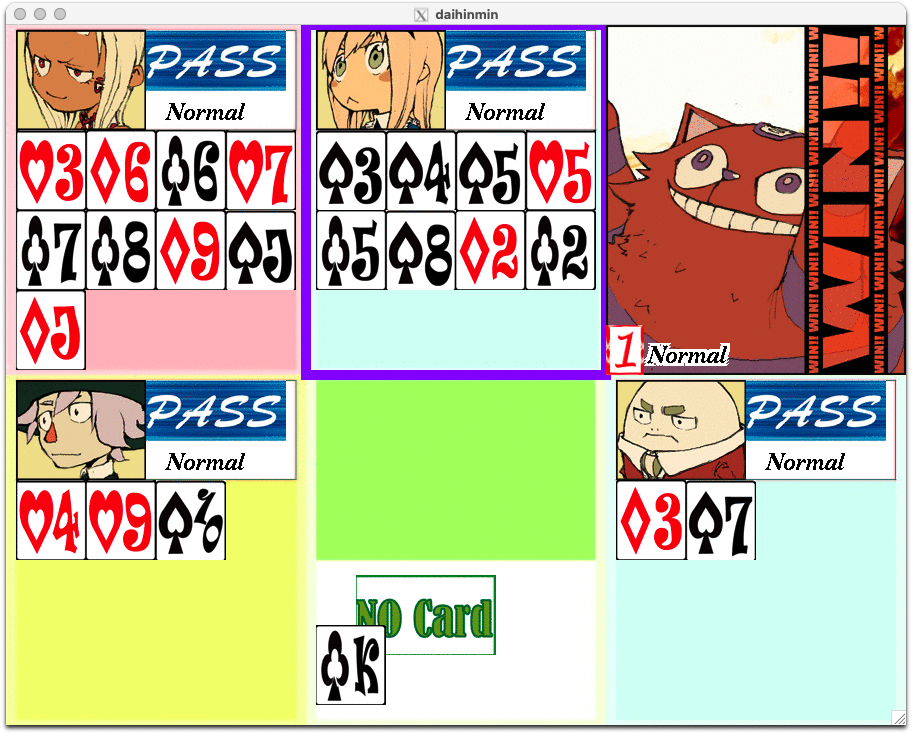
\includegraphics[width=0.8\textwidth]{./kadai9onzonpair.jpg}
  \caption{ペアや階段として出せるカードの温存}
\end{figure}

また、図5を見ると、場は縛りの状況で、「4」に対してそれ以上のカードは持っているが、ダイヤの9を出せるのに、ペアがあるため、カードを温存してそれ以降のカードを出す。
出されたカードがダイヤ10の1枚だあることがわかる。
\begin{figure}[h]
  \centering
  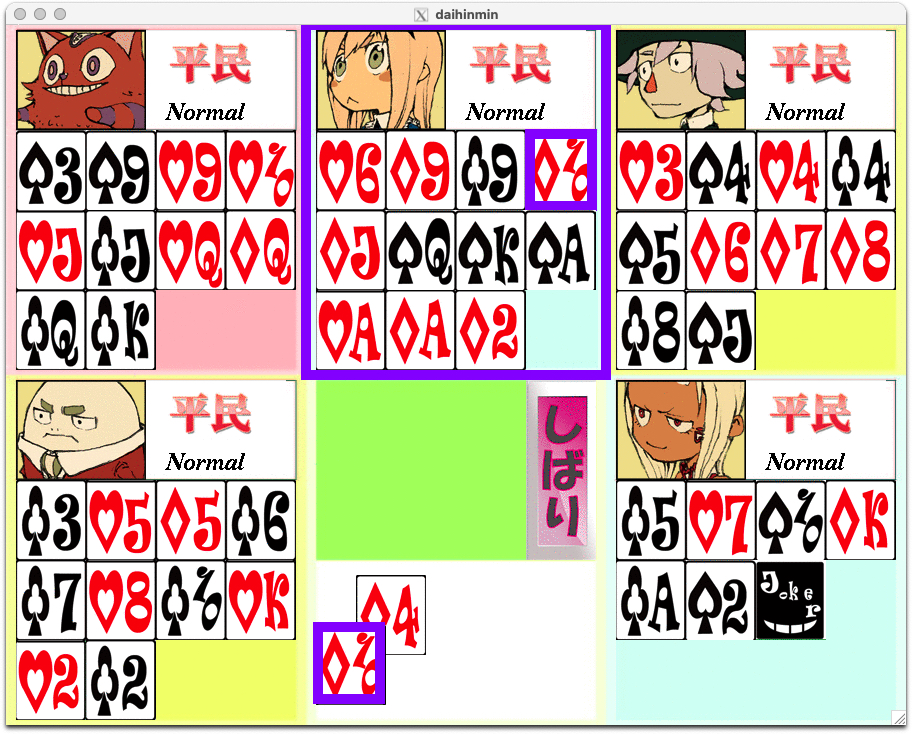
\includegraphics[width=0.8\textwidth]{./kadai9onzonpair2.jpg}
  \caption{ペアや階段として出せるカードの温存(2)}
\end{figure}

\newpage
\section{課題10(場が空の時のジョーカーを利用したペア提出機能と階段提出機能の実装)}
コンピュータ大貧民教育用クライアント(tndhmc-0.03.tar.gz)のディレクトリ src にある、 daihinmin.c などを改変し、
場が空の時のジョーカーを利用したペア出し機能および階段出し機能を実現した。\\

実装が完了したら、大貧民サーバを立ち上げゲームを実行し、場が空のとき、 ジョーカーを利用したペア出しや階段出しが
行われている様子がわかるスクリーンショットを取得して、図6と図7に示した。
また、実現したペア出し機能や階段出し機能について、考察を行った。\\

\noindent\textbf{場が空の時のジョーカーを利用したペアの提出}
\begin{lstlisting}[caption={daihinmin.c}]
  void make_info_table(int info_table[8][15], int info_j_table[8][15], int my_cards[8][15])
  {
    int i, j;
  
    clear_table(info_table);
    clear_table(info_j_table);
    for (i = 0; i < 4; i++)
    {
      for (j = 13; j > 0; j--)
      {
        if(my_cards[i][j] == 1){
          info_table[i][j] = info_table[i][j+1] + 1;
          info_j_table[i][j] = info_j_table[i][j+1] + 1;
        }
        else if(my_cards[i][j] == 0){
          info_table[i][j] = 0;
          info_j_table[i][j] = 0;
        }
      }
    }
  
    for (i = 0; i < 4; i++)
    {
      for (j = 1; j < 14; j++)
      {
        if(info_table[i][j] == 2){
          info_table[i][j] = 1;
          info_j_table[i][j] = 1;
        }
      }
    }
  
    for (i = 1; i <= 13; i++)
    {
      info_table[4][i] = my_cards[0][i] + my_cards[1][i] + my_cards[2][i] + my_cards[3][i];
    }
  
    if (my_cards[4][1] == 2){
      for(i = 1; i <= 13; i++){
        info_j_table[4][i] = info_table[4][i] + 1;
      }
    }
    else {
      for(i = 1; i <= 13; i++){
        info_j_table[4][i] = info_table[4][i];
      }
    }
  }

  int search_low_pair_wj(int dst_cards[8][15], int info_j_table[8][15], int my_cards[8][15]){
  int i, j, k;
  int sum;
  clear_table(dst_cards);
  for (i = 1; i < 14; i++){
    if(info_j_table[4][i] >= 2){
      sum = 0;
      for(j=0; j<4; j++){
        sum += my_cards[j][i];
      }
      while(sum < info_j_table[4][i]){
        for(k=0; k<4; k++){
          if(my_cards[k][i] == 0){
            dst_cards[k][i] = 2;
            sum++;
            break;
          }
        }
      }
      break;
    }
  }
  if(i <= 13){
    for(j=0; j <=3; j++){
      if(dst_cards[j][i] != 2)
        dst_cards[j][i] = my_cards[j][i];
    }
    print_info_table(dst_cards);
    return 1;
  }
  else
    return 0;
}
\end{lstlisting}

\begin{lstlisting}[caption={select\_cards.c}]
  void select_cards_free(int select_cards[8][15], int my_cards[8][15], state *field_status)
  {
    int info_table[8][15];
    int info_j_table[8][15];
  
    make_info_table(info_table, info_j_table, my_cards);
    printf("FREE\n");
    if (count_cards(select_cards) == 0)
      search_low_sequence(select_cards, info_table); // 手持ちの一番弱い階段を提出する
    if (count_cards(select_cards) == 0)
      search_low_pair_wj(select_cards, info_j_table, my_cards); // 手持ちの一番弱いペアを提出する
    if (count_cards(select_cards) == 0)
      search_low_card(select_cards, my_cards, 0); // 手持ちの一番弱いカードを単騎で提出する
  }
\end{lstlisting}
\section*{課題10の考察(ジョーカーを利用したペアの提出機能)}
\noindent ※ ジョーカーを利用した階段出しの提出機能は下に書いた。\\

まず、ソースコード6を見ると、make\_info\_table関数に info\_j\_table を追加した。これは、ジョーカーを持っている時の情報を格納するためである。
今の段階までの動作は、info\_table配列と同じだが、最後の方にジョーカーを持っているときは info\_j\_table 配列の5行目全てのカードの枚数を info\_tableの +1 にした。
一方、my\_cardsを読み取って、もしジョーカーを持っていない場合は、info\_j\_table 配列には info\_table 配列と同じ値を格納する。\\

次に、daihinmin.c の中に search\_low\_sequence\_wj 関数を新しく追加した。
この関数は、今から提出するカードの中にジョーカーが含まれる場合、その列のmy\_cards配列の中で0であるマスを2(ジョーカー)として dst\_cards 配列に埋めて提出される。
最後に、ソースコード7では、select\_cards\_free関数の中に search\_low\_pair\_wj 関数をsearch\_low\_pair関数の代わりに追加した。
そうすることで、ジョーカーを利用したペアの提出機能を実現できるようになった。\\

\noindent ジョーカーを利用したペアや階段の提出機能の実装結果を以下に示す。\\

\newpage

\section*{課題10ジョーカーを利用したペアの提出の実行結果}
場が空のときのジョーカーを利用したペアの提出機能の実装結果を図6に示す。図6を見ると、クローバーの「3」のペアが存在しないので、ジョーカーを利用してペアを提出していることがわかる。\\

\begin{figure}[h]
  \centering
  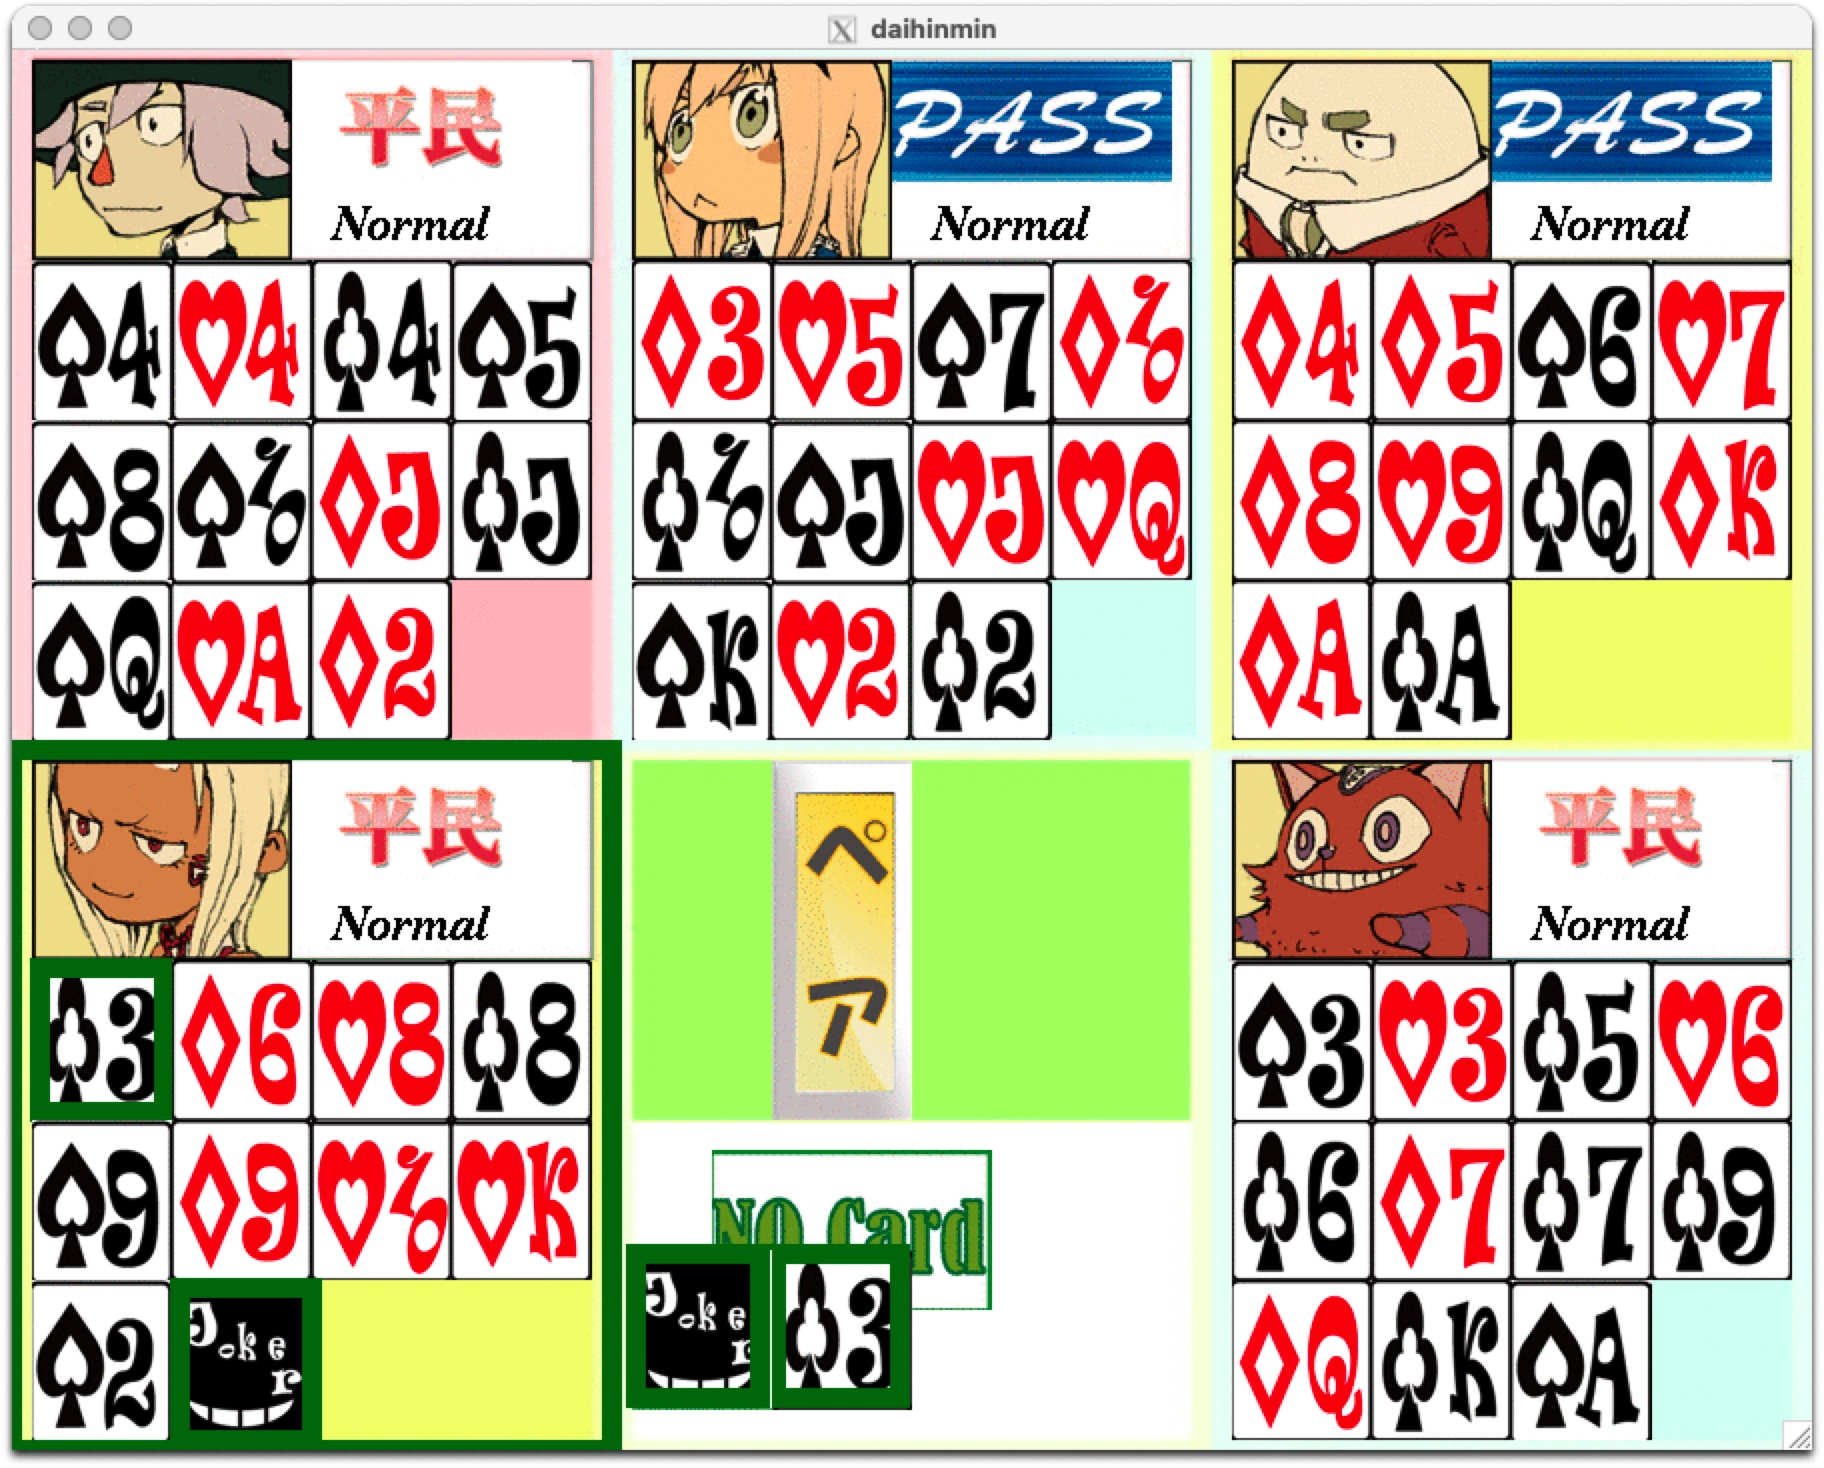
\includegraphics[width=0.8\textwidth]{./kadai10pairfree.jpg}
  \caption{場が空の時のジョーカーを利用したペア出しの実装結果}
\end{figure}

\noindent これをさらに改善して、ジョーカーを利用した階段の提出機能を実装した。そのソースコードを以下のソースコード8の通りで示す。\\

\newpage
\noindent\textbf{場が空の時のジョーカーを利用した階段の提出}
\begin{lstlisting}[caption={daihinmin.c}]
  void make_info_table(int info_table[8][15], int info_j_table[8][15], int my_cards[8][15])
  {
    int i, j;
    int joker_last_position;
    clear_table(info_table);
    clear_table(info_j_table);
    for (i = 0; i < 4; i++)
    {
      joker_last_position = 15;
      for (j = 13; j > 0; j--)
      {
        if(my_cards[i][j] == 1){
          info_table[i][j] = info_table[i][j+1] + 1;
          info_j_table[i][j] = info_j_table[i][j+1] + 1;
        }
        else if(my_cards[i][j] == 0){
          info_table[i][j] = 0;
          info_j_table[i][j] = joker_last_position - j;
          joker_last_position = j;
        }
      }
    }
  
    for (i = 0; i < 4; i++)
    {
      for (j = 1; j < 14; j++)
      {
        if(info_table[i][j] == 2){
          info_table[i][j] = 1;
        }
        if(info_j_table[i][j] == 2){
          info_j_table[i][j] = 1;
        }
      }
    }
  
    for (i = 1; i <= 13; i++)
    {
      info_table[4][i] = my_cards[0][i] + my_cards[1][i] + my_cards[2][i] + my_cards[3][i];
    }
  
    if (my_cards[4][1] == 2){
      for(i = 1; i <= 14; i++){
        info_j_table[4][i] = info_table[4][i] + 1;
      }
    }
    else {
      for(i = 1; i <= 14; i++){
        info_j_table[4][i] = info_table[4][i];
      }
    }
  }

  int search_low_sequence_wj(int dst_cards[8][15], int info_j_table[8][15], int my_cards[8][15]){
  int i, j, k;
  int search_flag = 0;
  clear_table(dst_cards);
  for (i=1; i<=13; i++)
  {
    for (j=0; j<4; j++)
    {
      if(info_j_table[j][i] >= 3){
        search_flag = 1;
        break;
      }
    }
    if (search_flag == 1) break;
  }
  if (i <= 13){
    for(k=0; k<info_j_table[j][i]; k++){
      if(my_cards[j][i+k] == 0){
        dst_cards[j][i+k] = 2;
      }
      else {
        dst_cards[j][i+k] = 1;
      }
    }
    return 1;
  } else {
    return 0;
  }
}
\end{lstlisting}

\begin{lstlisting}[caption={select\_cards.c}]
  void select_cards_free(int select_cards[8][15], int my_cards[8][15], state *field_status)
  {
    int info_table[8][15];
    int info_j_table[8][15];
  
    make_info_table(info_table, info_j_table, my_cards);
    printf("FREE\n");
    if (count_cards(select_cards) == 0)
      search_low_sequence_wj(select_cards, info_j_table, my_cards); // 手持ちの一番弱い階段を提出する
    if (count_cards(select_cards) == 0)
      search_low_pair_wj(select_cards, info_j_table, my_cards); // 手持ちの一番弱いペアを提出する
    if (count_cards(select_cards) == 0)
      search_low_card(select_cards, my_cards, 0); // 手持ちの一番弱いカードを単騎で提出する
  }
\end{lstlisting}

\section*{課題10の考察(ジョーカーを利用した階段の提出機能)}
まず、ソースコード8を見ると、make\_info\_table関数の info\_j\_table 配列をさらに改善した。
具体的には、info\_table配列と同じように、右から左にmy\_cards配列を確認して、もしそのマスが1の場合、そのマスの一つ右の値を +1 にして、そのマスに格納する。
一方、my\_cards配列の中が0の場合、そのマスの値をジョーカーの一番最後に使われた位置からの差を格納する。\\

なぜなら、ジョーカーが1枚しかないので、新しいマスにジョーカーを使う場合、最後に使ったジョーカーの位置を新しいマスに移動する必要があるからである。
また、make\_info\_tableの最後の方に、ソースコード6と同じく、my\_cards配列の中にジョーカーがある場合、info\_j\_table配列の中の値を +1 にして、それ以外の場合は、info\_j\_table配列の中の値をそのまま格納する。\\

次に、search\_low\_sequence\_wj関数を新しく作成して、ジョーカーを利用した階段の提出機能を実現している。
具体的には、ジョーカーが使われた場合、その列のmy\_cards配列の中で0であるカードを2(ジョーカー)に置き換えて提出される。\\
これもsearch\_low\_pair\_wj関数と同じように、ジョーカーを使って階段を提出するためである。
最後に、ソースコード9では、select\_cards\_free関数の中に search\_low\_sequence\_wj 関数をsearch\_low\_sequence関数の代わりに追加した。
そうすることで、ジョーカーを利用した階段の提出機能を実現できるようになった。\\

\newpage
\section*{課題10ジョーカーを利用した階段の提出の実行結果}
場が空のときのジョーカーを利用した階段の提出機能の実装結果を図7に示す。図7を見ると、ジョーカーを利用して階段を提出していることがわかる。
今の場合、ジョーカーはスペードの「4」として使われている。
出された階段はスペードの「3」、「4」、「5」、「6」であることがわかる。\\


\begin{figure}[h]
  \centering
  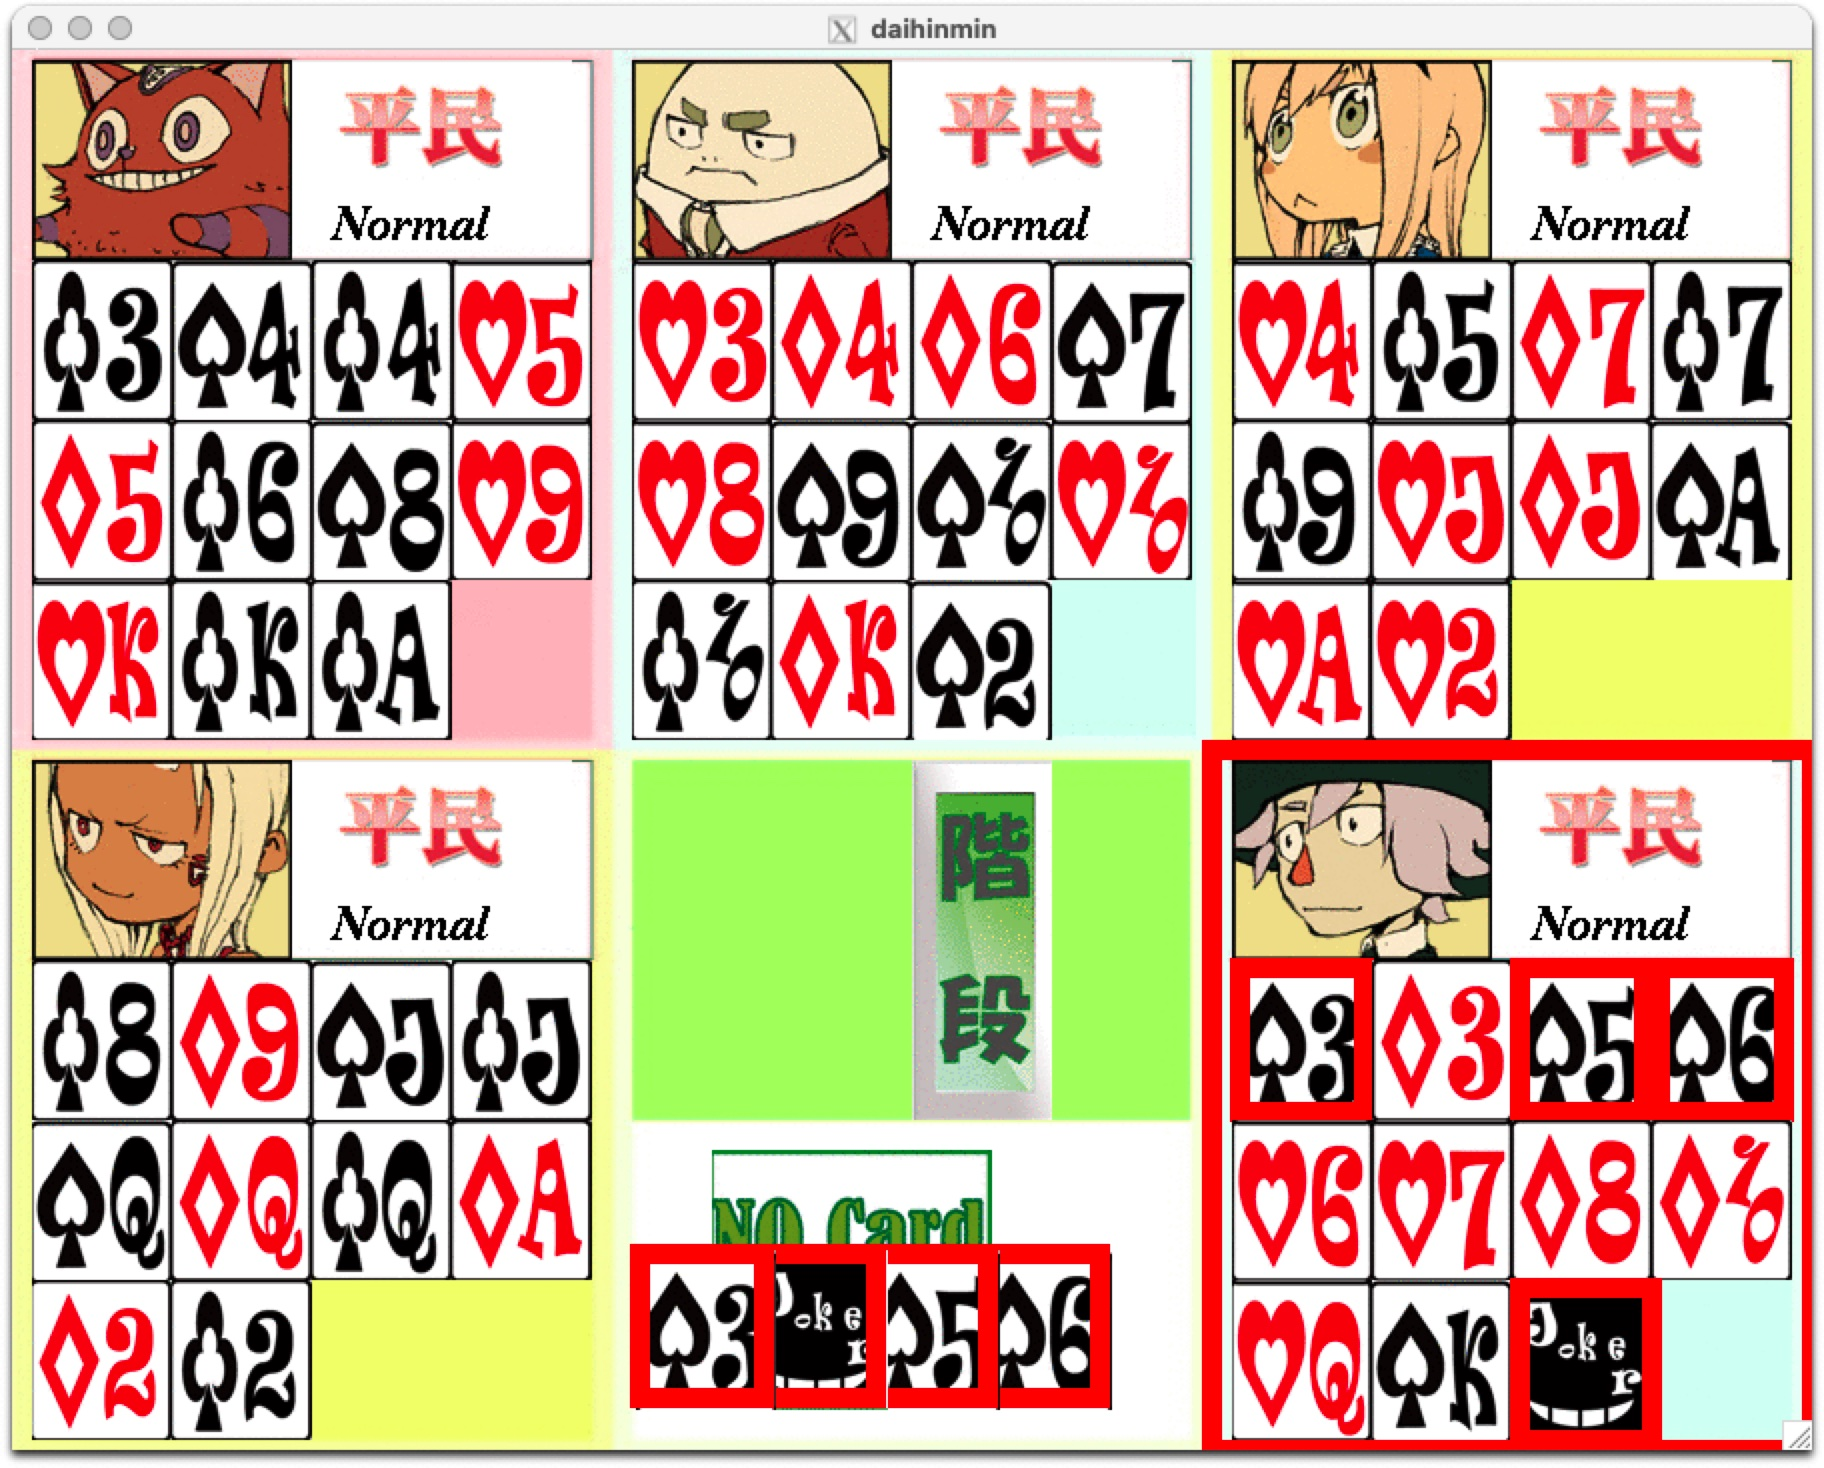
\includegraphics[width=0.8\textwidth]{./kadai10sequence.jpg}
  \caption{場が空の時のジョーカーを利用した階段出しの実装結果}
\end{figure}


\noindent 以上は4週目の課題レポートである。

\begin{thebibliography}{99}
  \bibitem{cite1} 第4回 コンピュータ大貧民(大貧民の実行とペア出し機能の実装), \\URL : \url{https://www.ied.inf.uec.ac.jp/text/laboratory/C/fourth_week/index04.html}
\end{thebibliography}
\end{document}
